%\section{Design and Development of the Artefacts}\label{sec:designArtefact}

%The artifact, which is intended to improve experimental research in behavioral research in data analytics, is to be implemented as a software component or application. In this step, a suitable architecture is developed based on the established requirements. For this purpose, the application is first fundamentally conceptualized. This involves analyzing possible technologies and the corresponding processes. The architecture is then implemented in practice on the basis of this basic conceptualization.

%\subsection{Process Conceptualization}\label{subsec:ProcessConcept}

%In order to effectively implement the requirements for the application, the processes described by the requirements and validated by the test cases are represented in the following swim lane diagrams. The goal of this is to illustrate the individual processes in a technology-independent manner. The reason for this is that the individual processes are initially presented in generalized form, irrespective of technological restrictions or limitations. Swim lane diagrams depict processes by showing business activities in relation to each other and how they are associated with each other (\cite{Caudle.2009}). A large part of the final functionalities can be divided into three different categories. Requirements that are concernd with functionalities and data related to the experiment itself, the individual participants and the interaction between these participants and the application through the \ac{ui}. The three lanes \enquote{Experiment Data}, \enquote{Participant Data} and \enquote{User} are representative for those three categories and data sources. The \enquote{User} lane shows the activities performed by the test subjects, the \enquote{Experimental Data} lane shows all activities that can be associated with the experimental setup, and the \enquote{Patricipant Data} lane shows all data and activities that are related to the test subjects. 

\section{Design and Development of the Artifacts}\label{sec:designArtefact}

The artifact, intended to improve experimental research in behavioral data analytics, is to be implemented as a software component or application. In this step, a suitable architecture is developed based on the established requirements. To achieve this, the application is first fundamentally conceptualized. This involves analyzing possible technologies and the corresponding processes. The architecture is then implemented in practice based on this initial conceptualization.

\subsection{Process Conceptualization}\label{subsec:ProcessConcept}

To effectively implement the requirements for the application, the processes described by the requirements and validated by the test cases are represented in the following swim lane diagrams. The goal is to illustrate the individual processes in a technology-independent manner. The reason for this is that the individual processes are initially presented in a generalized form, irrespective of technological restrictions or limitations. Swim lane diagrams depict processes by showing business activities in relation to each other and how they are associated with each other (\cite{Caudle.2009}). A significant portion of the final functionalities can be divided into three different categories: requirements related to functionalities and data pertaining to the experiment itself, the individual participants, and the interaction between these participants and the application through the \ac{ui}. The three lanes, \enquote{Experiment Data}, \enquote{Participant Data}, and \enquote{User}, represent these three categories and data sources. The \enquote{User} lane shows the activities performed by the test subjects, the \enquote{Experimental Data} lane shows all activities associated with the experimental setup, and the \enquote{Participant Data} lane shows all data and activities related to the test subjects.


\begin{figure}[htbp]
    \centering
    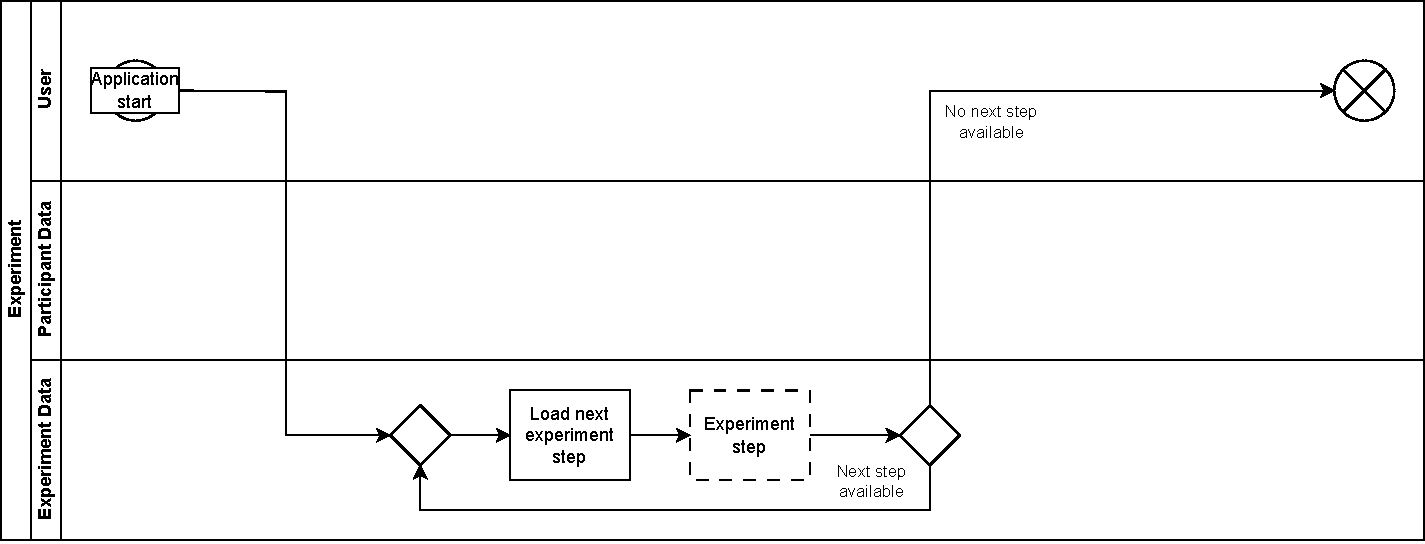
\includegraphics[width=0.99\textwidth, keepaspectratio]{content/05_design_and_dev_artefacts/ExperimentSwimLane.drawio.pdf}
    \caption{Experiment - Swim Lane}    
    \label{fig:experimentSwimLane}
\end{figure}

%Figure \ref{fig:experimentSwimLane} shows the basic structure of any experiment. The whole experiment is divided into different experiment steps, which are executed one after the other until the experiment is completed. The application is started first and then the first step of the experiment is executed. This could be for example an information message for the participants. After that the next step is executed if another step is available. If no further step is available, the experiment ends. This simple abstraction of an experiment concentrates on the essentials and thus allows the most flexible and adaptable construction kit for any experiment.
%According to the requirements a certain amount of standard \enquote{experiment steps} are developed for the artefact. These \enquote{standard steps} represent functionalities that are common between every imaginable experiment. In addition to this, the possibility should exist to create custom \enquote{experimental steps} in order to extend and customize the experiment. In the following five \enquote{standard experiment steps} based on the functional requirements are illustrated by the use of swim lane diagrams.  
%The dashed box \enquote{Experimental Step} of figur \ref{fig:experimentSwimLane} therefore represents one of the \enquote{standard steps} in figure \ref{fig:DataInputSwimLane}, \ref{fig:ChooseTestSubjectSwimLane}, \ref{fig:groupAllocationSwimLane}, \ref{fig:questionairSwimLane} and \ref{fig:infoScreenSwimLane}. For this reason, the graphics mentioned also begin and end in the \enquote{Experimental Repository} lane.

Figure \ref{fig:experimentSwimLane} shows the basic structure of any experiment. The whole experiment is divided into different experiment steps, which are executed one after the other until the experiment is completed. The application is started first, and then the first step of the experiment is executed. This could be, for example, an information message for the participants. After that, the next step is executed if another step is available. If no further step is available, the experiment ends. This simple abstraction of an experiment concentrates on the essentials and thus allows for the most flexible and adaptable construction kit for any experiment. According to the requirements, a certain number of standard \enquote{experiment steps} are developed for the artifact. These \enquote{standard steps} represent functionalities that are common to every imaginable experiment. In addition to this, the possibility should exist to create custom \enquote{experimental steps} in order to extend and customize the experiment. The following five \enquote{standard experiment steps} based on the functional requirements are illustrated using swim lane diagrams. The dashed box \enquote{Experimental Step} in Figure \ref{fig:experimentSwimLane} therefore represents one of the \enquote{standard steps} from Figures \ref{fig:DataInputSwimLane}, \ref{fig:ChooseTestSubjectSwimLane}, \ref{fig:groupAllocationSwimLane}, \ref{fig:questionairSwimLane}, and \ref{fig:infoScreenSwimLane}. For this reason, the mentioned graphics also begin and end in the \enquote{Experimental Repository} lane.


\begin{figure}[htbp]
    \centering
    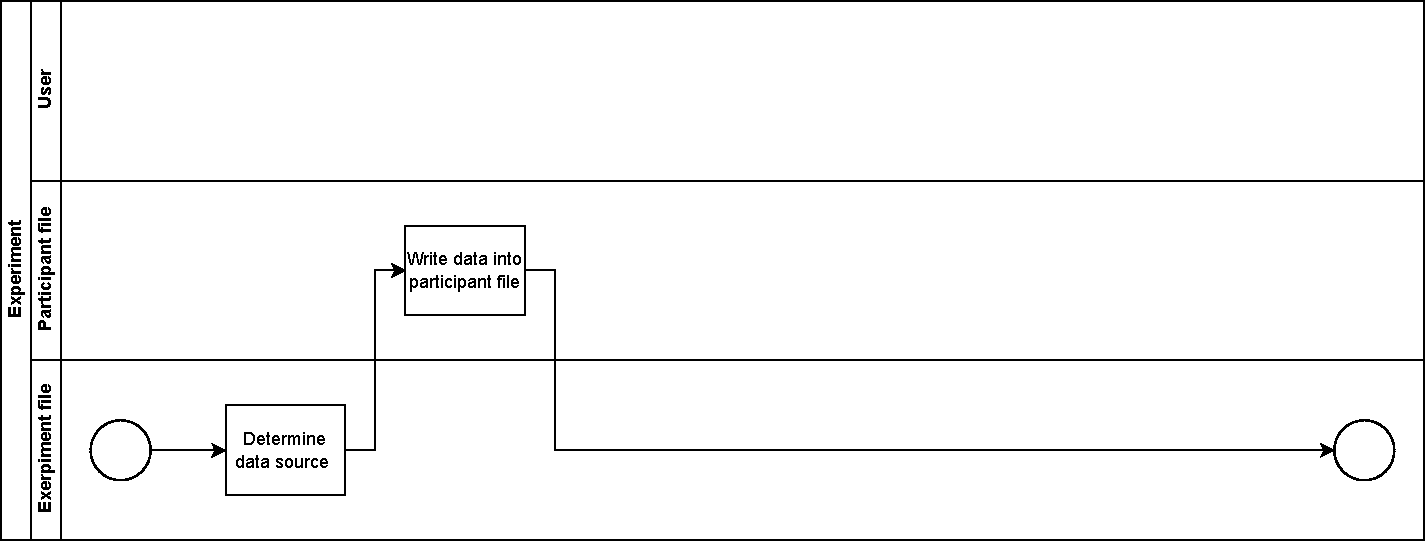
\includegraphics[width=0.99\textwidth, keepaspectratio]{content/05_design_and_dev_artefacts/DataInputSwimLane.drawio.pdf}
    \caption{Data Input Step - Swim Lane}    
    \label{fig:DataInputSwimLane}
\end{figure}

Figure \ref{fig:DataInputSwimLane} represents the process step of reading data from one or more sources. The assumption is that this data must first be processed or standardized before it can be meaningfully assigned to the participants and used within the experiment.

\begin{figure}[htbp]
    \centering
    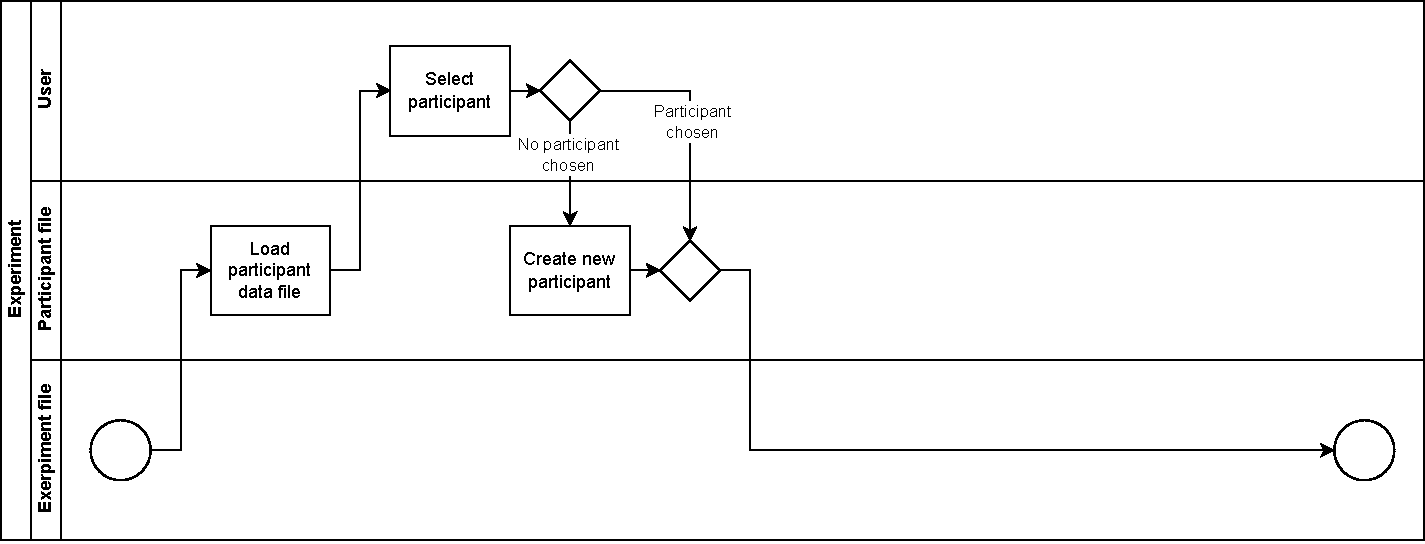
\includegraphics[width=0.99\textwidth, keepaspectratio]{content/05_design_and_dev_artefacts/ChooseTestSubjectSwimLane.drawio.pdf}
    \caption{Choose Test Subject Step - Swim Lane}    
    \label{fig:ChooseTestSubjectSwimLane}
\end{figure}

Figure \ref{fig:ChooseTestSubjectSwimLane} enables the mapping between the test subject and their \ac{id}, which will be used for the rest of the experiment.

\begin{figure}[htbp]
    \centering
    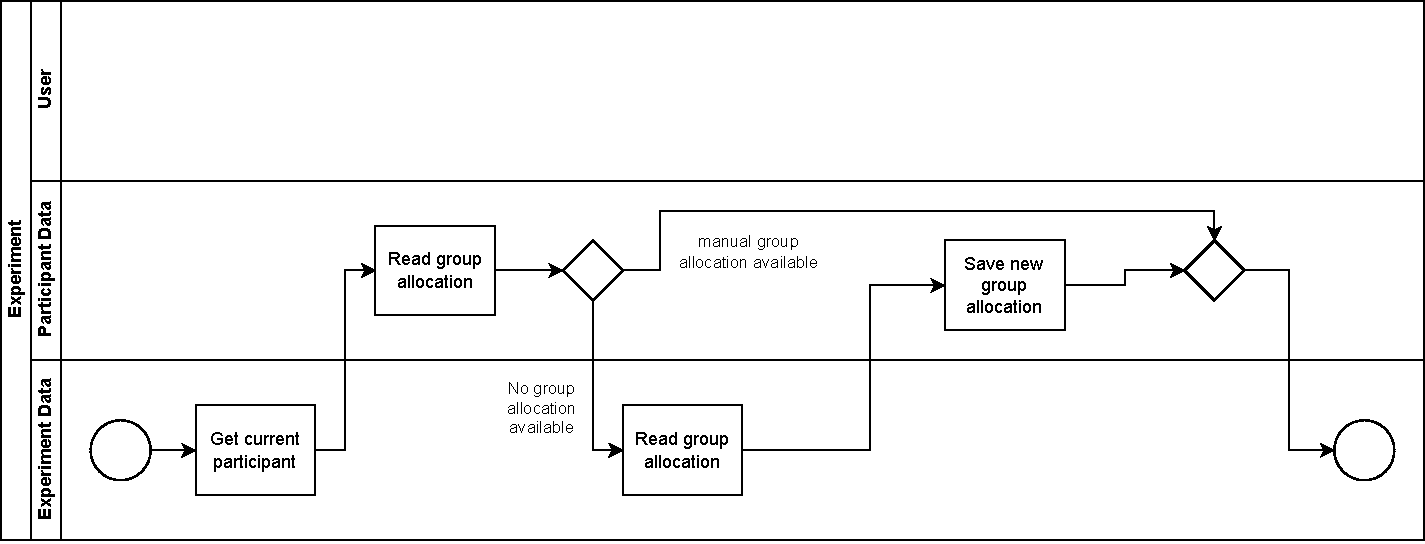
\includegraphics[width=0.99\textwidth, keepaspectratio]{content/05_design_and_dev_artefacts/GroupAllocationSwimLane.drawio.pdf}
    \caption{Group Allocation Step - Swim Lane}    
    \label{fig:groupAllocationSwimLane}
\end{figure}

%Figure \ref{fig:groupAllocationSwimLane} represents the process of assigning individual participants into groups. Participants can either be divided according to a predefined group, arbitrarily or according to certain criteria.

\newpage

Figure \ref{fig:groupAllocationSwimLane} represents the process of assigning individual participants to groups. Participants can be divided either according to a predefined group, arbitrarily, or according to certain criteria.


\begin{figure}[htbp]
    \centering
    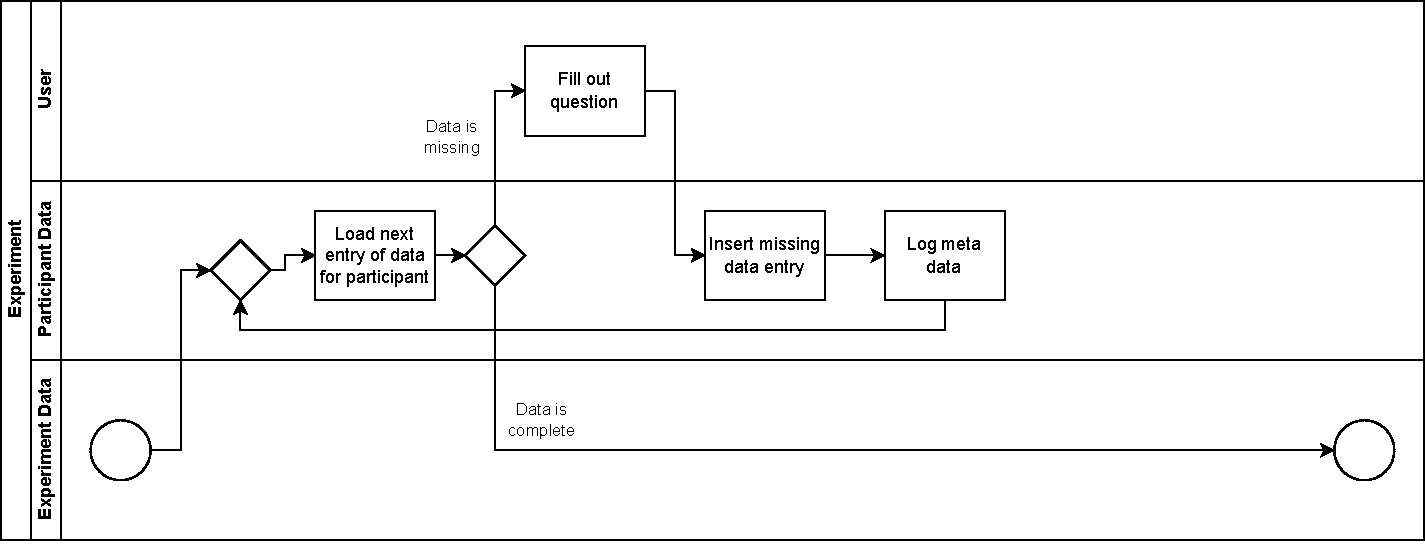
\includegraphics[width=0.99\textwidth, keepaspectratio]{content/05_design_and_dev_artefacts/QuestionairSwimLane.drawio.pdf}
    \caption{Questionnaire Step - Swim Lane}    
    \label{fig:questionairSwimLane}
\end{figure}

%Figure \ref{fig:questionairSwimLane} is used to complete missing information or data about the participants. For this purpose, test subjects are asked questions based on missing data entries corresponding to their \ac{id}. This process is conceptualized similarly to the general experiment setup, so that any number of questions or no question at all are displayed for completion, depending on the number of missing data points about a test subject. An example would be a participant thats age is missing in a dataset. An input field is automatically displayed for the participant to fill in the missing information about himself. If all data for a test subject is complete, nothing is displayed.

Figure \ref{fig:questionairSwimLane} is used to complete missing information or data about the participants. For this purpose, test subjects are asked questions based on missing data entries corresponding to their \ac{id}. This process is conceptualized similarly to the general experiment setup, so that any number of questions or no questions at all are displayed for completion, depending on the number of missing data points about a test subject. An example would be a participant whose age is missing in a dataset. An input field is automatically displayed for the participant to fill in the missing information about themselves. If all data for a test subject is complete, nothing is displayed.


\begin{figure}[htbp]
    \centering
    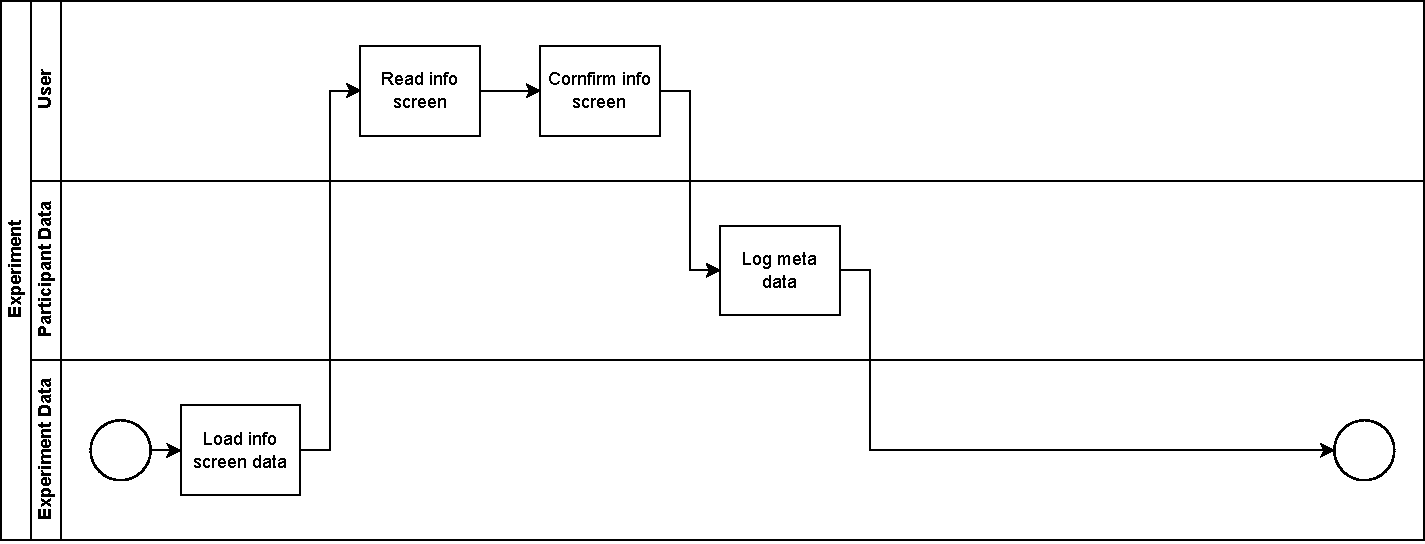
\includegraphics[width=0.99\textwidth, keepaspectratio]{content/05_design_and_dev_artefacts/InfoScreenSwimLane.drawio.pdf}
    \caption{Info Screen Step - Swim Lane}    
    \label{fig:infoScreenSwimLane}
\end{figure}

Figure \ref{fig:infoScreenSwimLane} displays information to the test subjects and can be used both as a means of notification during an experiment or just as a representation of information.

%\subsection{Technology Selection}

%In order to select appropriate technologies for the implementation of the application, the established requirements must be considered. It can be assumed that all functional requirements can be implemented by any modern programming language that is turing complete. The non-functional requirements N2.1 (Evaluation of Data), N2.2 (Vizualize Final Data), N6.1 (Multi-Source) are represented by the availability of various interfaces. Furthermore, the two non-functional requirements N1.2 (Time-Flexibility) and N5.1 (Monitoring of Study) are not relevant to the technology selection as these refer to the way the application is implemented and not its technological nature. This leaves requirements N1.1 (Distand Communication),  N3.1 (Simplicity), N4.1 (Reusable), N4.2 (Interoperability), N4.3 (Openness of Platform), N7.1 (Advanced User Interface) and the afformentioned availability of interfaces as requirements for selecting a suitable technology. In the following sections, various technologies and tools are presented that are intended to meet these requirements.

%Figure \ref{fig:infoScreenSwimLane} displays information to the test subjects and can be used both as a means of notification during an experiment or just as a representation of information.

\subsection{Technology Selection}

In order to select appropriate technologies for the implementation of the application, the established requirements must be considered. It can be assumed that all functional requirements can be implemented by any modern programming language that is Turing-Complete. The non-functional requirements N2.1 (Evaluation of Data), N2.2 (Visualize Final Data), N6.1 (Multi-Source) are represented by the availability of various interfaces. Furthermore, the two non-functional requirements N1.2 (Time-Flexibility) and N5.1 (Monitoring of Study) are not relevant to the technology selection as these refer to the way the application is implemented and not its technological nature. This leaves requirements N1.1 (Distant Communication), N3.1 (Simplicity), N4.1 (Reusable), N4.2 (Interoperability), N4.3 (Openness of Platform), N7.1 (Advanced User Interface), and the aforementioned availability of interfaces as requirements for selecting a suitable technology. In the following sections, technologies and tools are presented that are intended to meet these requirements.


%\subsubsection{Android and Android Studio}

%Android is an open source operating system for mobile devices which was first announced by Google in 2013. To date, Android has achieved a market share of over 90\% in the mobile sector and is the most used operating system over all, being used in almost every second device (\cite{statcounter.2023}, \cite{Richter.2019}). The standard development environment to develop Android is the \ac{ide} Android Studio, which supports a wide range of developer tools and functionalities. As an open source project and, due to its high distribution on various devices Android suits the openness of platform and interoperability requirement (\cite{Richter.2019}). Android applications are programs designed for touch inputs, which are specifically designed for mobile devices. However, as a widely used open source operating system, Android also supports other input options, advanced network capabilities and a variety of interfaces and extensions (\cite{Richter.2019}). Thus it can be assumed that the interface and distand communication requirements can be fulfilled through the usage of Android. The two programming languages that can be used to develop these Android applications are Java and Kotlin. Android applications can be tested either directly on an Android device or on a variety of virtual devices integrated in Android Studio, which further facilitates the development of said applications (\cite{Richter.2019}). As a mobile operating system, one of Android's main focuses is the user interface as an input function, in addition to network functionalities and a variety of interfaces. Android also has a wide range of design guidelines, interface functionalities and is updated at very regular intervals (\cite{statista.2023}, \cite{Richter.2019}). Due to these regular updates, the widespread use of Android, the focus on \ac{ui} intensive use cases and the broad functionalities like network capabilities and a the support for different interfaces, it can be assumed that an application developed in Android fullfills the afformentioned requirements.

%\subsubsection{Java}

%Since 2009 Java is part of the product portfolio of Oracle Corporation. Java is an object-oriented programming language, which makes it an universally applicable and robust programming language (\cite{Ullenboom.2017}). Unlike many other programming languages, one of the special features of Java is its platform independence. Most programming languages use a compiler or interpreter to translate program code into byte code, which varies depending on the hardware and can only be executed on the appropriate processors. Java avoids this limitation by first having a compiler translate the Java program code into byte code, which is then executed via an interpreter in a virtual environment which is called \ac{jvm}. In this way, Java code can theoretically be executed on any system (\cite{Ullenboom.2017}). This makes Java not only a programming language but also a runtime system, which is made clear by the naming of the Java Platform by Oracle. The Java Platform supports beside Java itself also the execution of some other programming languages as for example Kotlin (\cite{kotlinlang.2023}). Due to this fact, Java is especially suitable for the implementation of the artefact based on the requirements N4.1 (Reusable) and N4.2 (Interoperability). Java also supports a variety of programming concepts through standard libraries. These include data structures, string processing, date/time processing, graphical interfaces, input/output, network operations, threads and more (\cite{Ullenboom.2017}), which ensures the N1.1 (Distand Communication) requirement and the availability of interfaces. The Java runtime environment also enables fast code execution and comes with various utilities such as a garbage collector and output name handlers. The syntax of Java is generally considered to be very easy to understand and beginner-friendly (\cite{Ullenboom.2017}), fulfilling the requirement N3.1 (Simplicity). In addition to technical aspects, Java is also Open-Source, extremely widespread, popular and a variety of literature for it is available (\cite{Ullenboom.2017}), which generally indicates an openness of platform (Requirement N4.3 Openness of Platform) and convenient to develope code (N3.1 (Simplicity)). Disadvantages of Java, which are also mentioned for the sake of completeness, mainly relate to very specific platform-dependent use cases. Since Java was developed as a general-purpose programming language and platform-independent, it is very difficult to access hardware or drivers directly. However, these limitations are very specific and therefore irrelevant in the context of this thesis (\cite{Ullenboom.2017}). 

\subsubsection{Android and Android Studio}

Android is an open-source operating system for mobile devices, which was first announced by Google in 2013. To date, Android has achieved a market share of over 90\% in the mobile sector and is the most used operating system overall, being used in almost every second device (\cite{statcounter.2023}, \cite{Richter.2019}). The standard development environment to develop Android applications is the \ac{ide} Android Studio, which supports a wide range of developer tools and functionalities. As an open-source project and, due to its high distribution on various devices, Android suits the N4.3 \enquote{Openness of Platform} and N4.2 \enquote{Interoperability} requirement (\cite{Richter.2019}). Android applications are programs designed for touch inputs, specifically for mobile devices. However, as a widely used open-source operating system, Android also supports other input options, advanced network capabilities, and a variety of interfaces and extensions (\cite{Richter.2019}). Thus, it can be assumed that the interface and N1.1 \enquote{Distant Communication} requirements can be fulfilled through the usage of Android. The two programming languages that can be used to develop these Android applications are Java and Kotlin. Android applications can be tested either directly on an Android device or on a variety of virtual devices integrated into Android Studio, which further facilitates the development of said applications (\cite{Richter.2019}). As a mobile operating system, one of Android's main focuses is the \ac{ui} as an input function, in addition to network functionalities and a variety of interfaces. Android also has a wide range of design guidelines, interface functionalities, and is updated at regular intervals (\cite{statista.2023}, \cite{Richter.2019}). Due to these regular updates, the widespread use of Android, the focus on \ac{ui}-intensive use cases, and the broad functionalities like network capabilities and support for different interfaces, it can be assumed that an application developed in Android fulfills the aforementioned requirements.

\subsubsection{Java}

Since 2009, Java has been part of the product portfolio of Oracle Corporation. Java is an object-oriented programming language, making it a universally applicable and robust programming language (\cite{Ullenboom.2017}). Unlike many other programming languages, one of the special features of Java is its platform independence. Most programming languages use a compiler or interpreter to translate program code into bytecode, which varies depending on the hardware and can only be executed on the appropriate processors. Java avoids this limitation by first having a compiler translate the Java program code into bytecode, which is then executed via an interpreter in a virtual environment called \ac{jvm}. In this way, Java code can theoretically be executed on any system (\cite{Ullenboom.2017}). This makes Java not only a programming language but also a runtime system, which is made clear by the naming of the Java Platform by Oracle. The Java Platform supports, besides Java itself, the execution of some other programming languages, such as Kotlin (\cite{kotlinlang.2023}). Due to this fact, Java is especially suitable for the implementation of the artifact based on the requirements N4.1 (Reusable) and N4.2 (Interoperability). Java also supports a variety of programming concepts through standard libraries. These include data structures, string processing, date/time processing, graphical interfaces, input/output, network operations, threads, and more (\cite{Ullenboom.2017}), which ensures the N1.1 (Distant Communication) requirement and the availability of interfaces. The Java runtime environment also enables fast code execution and comes with various utilities such as a garbage collector and output name handlers. The syntax of Java is generally considered to be easy to understand and beginner-friendly (\cite{Ullenboom.2017}), fulfilling the requirement N3.1 (Simplicity). In addition to technical aspects, Java is also open-source, extremely widespread, popular, and a variety of literature is available for it (\cite{Ullenboom.2017}), which generally indicates openness of the platform (Requirement N4.3 Openness of Platform) and convenience in developing code (N3.1 Simplicity). Disadvantages of Java, which are also mentioned for the sake of completeness, mainly relate to specific platform-dependent use cases. Since Java was developed as a general-purpose programming language and is platform-independent, it is difficult to access hardware or drivers directly (\cite{Ullenboom.2017}). However, these limitations are specific and therefore irrelevant in the context of this thesis.  



%\subsection{System Architecture Development}

%Overall, it can be summarized that the non-functional requirements, which consider properties of the system, are completely fulfilled by using the Android operating system in combination with the Java programming language. In general, most of the requirements could already be met by both Android and Java alone, so the combination of the two provides a solid foundation for meeting the requirements. However, as already noted in Section \ref{subsec:reqSpec}, the fulfillment of the non-functional requirements is by no means a binary state, but can be partly of a subjective nature, which is why no test cases could be set up for some requirements. Taking the above arguments into account, and especially the extremely wide distribution of the Android operating system, the technical combination of Android and Java for the implementation of the artifact is considered an appropriate choice. 
%For this reason, the artifact is implemented in the form of a mobile Android application. The Android API 24 (Android 7.0, Nougat) is used for this implementation. This Android version was chosen because it has all the interfaces and functionalities needed for the development of the artifact and an application developed on this version runs on about 95.4\% of all Android devices. At the same time, the application can easily be ported to a new version if newer features are needed for the implementation of an experiment (\cite{Google.2023}).

%The recommended architecture for an Android application consists of three layers, the \ac{ui} layer, the domain layer, and the data layer. The \ac{ui} layer displays application data and the application itself to the user.
%The domain layer is optional. It is used for abstraction and structuring of the data layer and is recommended above all if the application is to represent very complex business cases or the application must be designed to be very reusable (\cite{Google.2023}). Due to the requirements N4.1 (Reusable), a domain layer is therefore used in the conceptualized architecture. Classes in this layer are usually called use cases or interactions and always represent a single functionality. For example, the output of the time could be a functionality that must be used by several components. This functionality would then be represented by a \textit{GetTimeUseCase} class. The data layer contains the data and business logic of the application (\cite{Google.2023}). This layer defines to what extent data is processed, modified or stored. It is also divided into two parts, the repositories and the data sources (\cite{Google.2023}). The repositories are responsible for exposing the data to the rest of the application, to centralize changes to the data and to resolve conflicts between data sources. A repository can contain zero or multiple data sources. The repositories also contain the business logic and abstract the data sources from the rest of the application. Each data source is represented by one data source class which is the link between the system for data operations and the application. Sources for these data sources could be a file, a network or a local data base (\cite{Google.2023}).
%In the following, the concrete implementation of the architecture of the artifact is presented. The technical components are divided into the \ac{ui} layer, the domain layer and the data layer. 

\subsection{System Architecture Development}

Overall, it can be summarized that the non-functional requirements, which consider properties of the system, are completely fulfilled by using the Android operating system in combination with the Java programming language. In general, most of the requirements could already be met by both Android and Java alone, so the combination of the two provides a solid foundation for meeting the requirements. However, as already noted in section \ref{subsec:reqSpec}, the fulfillment of the non-functional requirements is by no means a binary state, but can be partly of a subjective nature, which is why no test cases could be set up for some requirements. Taking the above arguments into account, and especially the extremely wide distribution of the Android operating system, the technical combination of Android and Java for the implementation of the artifact is considered an appropriate choice. For this reason, the artifact is implemented in the form of a mobile Android application. The Android API 24 (Android 7.0, Nougat) is used for this implementation. This Android version was chosen because it has all the interfaces and functionalities needed for the development of the artifact, and an application developed on this version runs on about 95.4\% of all Android devices. At the same time, the application can easily be ported to a new version if newer features are needed for the implementation of an experiment (\cite{Google.2023}). 

The recommended architecture for an Android application consists of three layers: the \ac{ui} layer, the domain layer, and the data layer. The \ac{ui} layer displays application data and the application itself to the user. The domain layer is optional. It is used for abstraction and structuring of the data layer and is recommended above all if the application is to represent complex business cases or the application must be designed to be reusable (\cite{Google.2023}). Due to the requirements N4.1 (Reusable), a domain layer is therefore used in the conceptualized architecture. Classes in this layer are usually called use cases or interactions and always represent a single functionality. For example, the output of the time could be a functionality that must be used by several components. This functionality would then be represented by a \textit{GetTimeUseCase} class. The data layer contains the data and business logic of the application (\cite{Google.2023}). This layer defines to what extent data is processed, modified, or stored. It is also divided into two parts: the repositories and the data sources (\cite{Google.2023}). The repositories are responsible for exposing the data to the rest of the application, centralizing changes to the data, and resolving conflicts between data sources. A repository can contain zero or multiple data sources. The repositories also contain the business logic and abstract the data sources from the rest of the application. Each data source is represented by one data source class, which is the link between the system for data operations and the application. Sources for these data sources could be a file, a network, or a local database (\cite{Google.2023}).
In the following, the concrete implementation of the architecture of the artifact is presented. The technical components are divided into the \ac{ui} layer, the domain layer, and the data layer.


%\subsubsection{Data Layer}

%The individual data sources are masked from the rest of the application by the so-called repositories. In principle, however, a large number of different data sources can be used. Among others, local files, database systems or network storage. The number of data sources can vary between none and any number. The individual data sources depend on the respective experiment. For this reason, a simple local CSV file is used as a placeholder for different data sources. This is done for the sake of simplicity, in an actual experiment this placeholder file can then be replaced by any other combination of data sources.
%The data layer as a whole corresponds to the \textit{Particpant Data} and \textit{Epxeriment Data} lanes from the previously defined processes in the swim lane diagrams \ref{fig:experimentSwimLane}, \ref{fig:DataInputSwimLane}, \ref{fig:ChooseTestSubjectSwimLane}, \ref{fig:groupAllocationSwimLane}, \ref{fig:questionairSwimLane} and \ref{fig:infoScreenSwimLane} as these contain the business logic for elements associated with the experiment itself and the test subjects respectively. For this reason and in order to clearly abstract the standard data sources of the artefact from potential data sources that get implemented within experiments two repositories called \textit{ParticipantRepository} and \textit{ExperimentRepository} are implemented. 

%The Android development scheme for application specifies that all processing and unification of data should take place exclusively in the data layer. For this reason, all processes and activities involving data sources must be implemented in this layer. This concerns only the unification and standardization of data sources. Logic and the modification of data is performed in the domain layer. For this reason, the \enquote{Data Input Step} illustrated in swim lane figure \ref{fig:DataInputSwimLane}, which includes the reading and standardization of data, is not implemented as a single process step of an experiment but in the course of the development of the data layer. Thus, this step is the only one which must be implemented in the course of the development of the experiment. In the actual technical implementation, the data of the experiment and the participants is passed on to the repositories above it and the domain layer in the form of a so-called entity classes. The corresponding data and properties are contained as attributes in these entity classes and can be modified via getter and setter methods. The persistence of the data is ensured by the singleton principle, which is applied to the respective repositories.

%\subsubsection{Domain Layer}

%The domain layer is an optional layer that encapsulates complex business logic or logic that needs to be reused frequently (\cite{Google.2023}). Since it is not known to what extent the individual elements will be used in an experiment and a special focus is placed on the reusability of the individual components, this optional layer is implemented in the artifact. Further advantages resulting from the use of a domain layer are the avoidance of duplicated code, the improved readability of the architecture, an improvement in the testability of the application and the avoidance of large classes by splitting the tasks (\cite{Google.2023}). The domain layer classes are accessed in the same way by the \ac{ui} as repositories of the data layer are accessed. A simple non related example of a domain layer class would be to request the addresses of the best authors of the year. In this example there would be two data sources with repositories, one for authors and their addresses and another one containing the best selling books of the year. A domain layer class would hide access to these two repositories and the complex logic of determining the addresses of the best authors of the year from the rest of the application. To keep the classes of the domain layer simple it is adviced that each class should contain only a single functionality and should not contain mutable data (\cite{Google.2023}). These individual functions are also called use cases. Use cases (Domain Layer classes) can call each other and can be hierarchically dependent with each other within the domain layer as needed. Since one use case is supposed to represent one function at a time, a domain layer class (or use case) is created for each function or action that appears in one of the process swim lane diagrams in the \textit{Experiment Data} and \textit{Participant Data} lane from section \ref{subsec:ProcessConcept}. Entire processes (swim lanes) that do not contain user input are also illustrated by these domain layer use case classes. This case applies to the process in Swim Lane Diagram \ref{fig:groupAllocationSwimLane}, which is why it is modeled as a Use Case in the Domain Layer.
%A detailed view of the derived use cases is included in appendix \ref{appendix:C}. For the implementation of the individual UseCases, a Java class is created for each case, which contains the corresponding logic and the UseCase calls as corresponding interfaces through methods.

\subsubsection{Data Layer}

The individual data sources are masked from the rest of the application by the so-called repositories. In principle, however, a large number of different data sources can be used. Among others, local files, database systems, or network storage. The number of data sources can vary from none to any number. The individual data sources depend on the respective experiment. For this reason, a simple local \ac{csv} file is used as a placeholder for different data sources. This is done for the sake of simplicity; in an actual experiment, this placeholder file can then be replaced by any other combination of data sources. The data layer as a whole corresponds to the \textit{Participant Data} and \textit{Experiment Data} lanes from the previously defined processes in the swim lane diagrams \ref{fig:experimentSwimLane}, \ref{fig:DataInputSwimLane}, \ref{fig:ChooseTestSubjectSwimLane}, \ref{fig:groupAllocationSwimLane}, \ref{fig:questionairSwimLane}, and \ref{fig:infoScreenSwimLane}. These lanes contain the business logic for elements associated with the experiment itself and the test subjects, respectively. For this reason, and in order to clearly abstract the standard data sources of the artifact from potential data sources that get implemented within experiments, two repositories called \textit{ParticipantRepository} and \textit{ExperimentRepository} are implemented. The Android development scheme for the application specifies that all processing and unification of data should take place exclusively in the data layer. For this reason, all processes and activities involving data sources must be implemented in this layer. This concerns only the unification and standardization of data sources. Logic and the modification of data are performed in the domain layer. For this reason, the \enquote{Data Input Step} illustrated in swim lane figure \ref{fig:DataInputSwimLane}, which includes the reading and standardization of data, is not implemented as a single process step of an experiment but in the course of the development of the data layer. Thus, this step is the only one which must be implemented in the course of the development of the experiment. In the actual technical implementation, the data of the experiment and the participants are passed on to the repositories above it and the domain layer in the form of so-called entity classes. The corresponding data and properties are contained as attributes in these entity classes and can be modified via getter and setter methods. The persistence of the data is ensured by the singleton principle, which is applied to the respective repositories.

\subsubsection{Domain Layer}

The domain layer is an optional layer that encapsulates complex business logic or logic that needs to be reused frequently (\cite{Google.2023}). Since it is not known to what extent the individual elements will be used in an experiment, and a special focus is placed on the reusability of the individual components, this optional layer is implemented in the artifact. Further advantages resulting from the use of a domain layer are the avoidance of duplicated code, the improved readability of the architecture, an improvement in the testability of the application, and the avoidance of large classes by splitting the tasks (\cite{Google.2023}). The domain layer classes are accessed in the same way as repositories of the data layer are accessed by the \ac{ui}. A simple unrelated example of a domain layer class would be to request the addresses of the best authors of the year. In this example, there would be two data sources with repositories, one for authors and their addresses and another one containing the best-selling books of the year. A domain layer class would hide access to these two repositories and the complex logic of determining the addresses of the best authors of the year from the rest of the application. To keep the classes of the domain layer simple, it is advised that each class should contain only a single functionality and should not contain mutable data (\cite{Google.2023}). These individual functions are also called use cases. Use cases (Domain Layer classes) can call each other and can be hierarchically dependent on each other within the domain layer as needed. Since one use case is supposed to represent one function at a time, a domain layer class (or use case) is created for each function or action that appears in one of the process swim lane diagrams in the \textit{Experiment Data} and \textit{Participant Data} lanes from section \ref{subsec:ProcessConcept}. Entire processes (swim lanes) that do not contain user input are also illustrated by these domain layer use case classes. This case applies to the process in swim lane diagram \ref{fig:groupAllocationSwimLane}, which is why it is modeled as a use case in the Domain Layer. A detailed view of the derived use cases is included in appendix \ref{appendix:C}. For the implementation of the individual use cases, a Java class is created for each case, which contains the corresponding logic, and the use case calls corresponding interfaces through methods.


%\subsubsection{User Interface Layer}

%The concept of graphical user interfaces is implemented in Android via so-called activities, which represent special classes that contain a temporary data state and the \ac{ui} elements the user interacts with. While the start of an application in regular Java applications takes place via a \textit{main()} method, an Android application initiates code via these activities. The Android developer documentation describes an activity as \enquote{[...] entry point for an application's interaction with the user} (\cite{Google.2023}). The required \ac{ui} elements of the application are generated in these activity. An activity corresponds to a single screen of an application. Application can contain several different \ac{ui} screens and thus several different activities. Activities can also call other activities and navigate to them as desired. An application is therefore a sequence of different activities that represent different screens. Usually, an activity serves as the entry point to the application. This activty, also called the main activty, is the first screen that is shown when the application is started. Although Activities together form a complete application, Activities are only very superficially connected to each other. Basically, each activity is a replaceable, self-contained component that can be called in any order. This reusability and separation makes Activities the perfect foundation to implement the individual \enquote{experiment steps} that contain user interactions described in Section \ref{subsec:ProcessConcept}. Based on this fact and the fact that an Activity corresponds to a \ac{ui}, a separate Activity is designed for each process step from Section \ref{subsec:ProcessConcept} that contains user interactions. The three experiment steps, which include user inputs are the \textit{choose test subject}, \textit{questionair} and \textit{info screen} step, depicted in figure \ref{fig:ChooseTestSubjectSwimLane}, \ref{fig:questionairSwimLane} and \ref{fig:infoScreenSwimLane}. Figure \ref{fig:uiPrototypeArtefact} depicts these three use cases as a \ac{ui} prototype. Figure \ref{subfig:chooseTestSubject} represents the process step of choosing a test subject depicted in figure \ref{fig:ChooseTestSubjectSwimLane}. Figure \ref{subfig:Questionair} represents the process step of letting the test subject answer questions depicted in figure \ref{fig:questionairSwimLane}. Figure \ref{subfig:InfoScreen}  represents the process step of showing information to the test subject depicted in figure \ref{fig:infoScreenSwimLane}. The three \ac{ui} sketches show the basic division of \ac{ui} elements, to which the actual implementation of the activities is oriented. Furthermore, other custom steps from an experiment that contain user interactions would also be implemented using Activities. In this way, the reusability and separation of the individual experiment steps is guaranteed.

\subsubsection{User Interface Layer}

The concept of a graphical \ac{ui} is implemented in Android via so-called activities, which represent special classes that contain a temporary data state and the \ac{ui} elements the user interacts with. While the start of an application in regular Java applications takes place via a \textit{main()} method, an Android application initiates code via these activities. The Android developer documentation describes an activity as \enquote{[...] entry point for an application's interaction with the user} (\cite{Google.2023}). The required \ac{ui} elements of the application are generated in these activities. An activity corresponds to a single screen of an application. An application can contain several different \ac{ui} screens and thus several different activities. Activities can also call other activities and navigate to them as desired. An application is therefore a sequence of different activities that represent different screens. Usually, an activity serves as the entry point to the application. This activity, also called the main activity, is the first screen that is shown when the application is started. Although activities together form a complete application, activities are only superficially connected to each other. Basically, each activity is a replaceable, self-contained component that can be called in any order. This reusability and separation make activities the perfect foundation to implement the individual \enquote{experiment steps} that contain user interactions described in section \ref{subsec:ProcessConcept}. Based on this fact and the fact that an activity corresponds to a \ac{ui}, a separate activity is designed for each process step from section \ref{subsec:ProcessConcept} that contains user interactions. The three experiment steps, which include user inputs, are the \textit{Choose Test Subject}, \textit{Questionnaire}, and \textit{Info Screen} steps, depicted in Figures \ref{fig:ChooseTestSubjectSwimLane}, \ref{fig:questionairSwimLane}, and \ref{fig:infoScreenSwimLane}. Figure \ref{fig:uiPrototypeArtefact} depicts these three use cases as a \ac{ui} prototype. Figure \ref{subfig:chooseTestSubject} represents the process step of choosing a test subject depicted in figure \ref{fig:ChooseTestSubjectSwimLane}. Figure \ref{subfig:Questionair} represents the process step of letting the test subject answer questions depicted in Figure \ref{fig:questionairSwimLane}. Figure \ref{subfig:InfoScreen} represents the process step of showing information to the test subject depicted in Figure \ref{fig:infoScreenSwimLane}. The three \ac{ui} sketches show the basic division of \ac{ui} elements to which the actual implementation of the activities is oriented. Furthermore, other custom steps from an experiment that contain user interactions would also be implemented using activities. In this way, the reusability and separation of the individual experiment steps are guaranteed. The individual activities only hold a temporary dataset of information that is displayed or required in the \ac{ui}. As already explained, all other business logic is outsourced to the domain layer. The domain layer can be called and consumed by all activities at any time.



\begin{figure}
    \centering
    \begin{subfigure}[b]{0.25\textwidth}
        \centering
        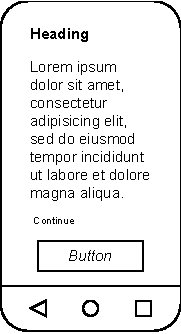
\includegraphics[width=\textwidth]{content/05_design_and_dev_artefacts/ActivityInfoScreen.drawio.pdf}
        \caption{Info Screen}
        \label{subfig:InfoScreen}
    \end{subfigure}
    \hspace{1cm}
    \begin{subfigure}[b]{0.25\textwidth}
        \centering
        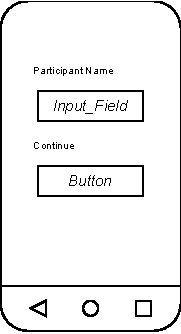
\includegraphics[width=\textwidth]{content/05_design_and_dev_artefacts/ActivityParticipantChoose.drawio.pdf}
        \caption{Choose Test Subject}
        \label{subfig:chooseTestSubject}
    \end{subfigure}
    \hspace{1cm}
    \begin{subfigure}[b]{0.25\textwidth}
        \centering
        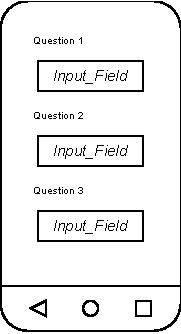
\includegraphics[width=\textwidth]{content/05_design_and_dev_artefacts/ActivityQuestionair.drawio.pdf}
        \caption{Questionnaire}
        \label{subfig:Questionair}

    \end{subfigure}
       \caption{User Interface Prototype of Artifact}
       \label{fig:uiPrototypeArtefact}
\end{figure}

%The individual activities only hold a temporary data set of information that is displayed or required in the \ac{ui}. As already explained, all other business logic is outsourced to the domain layer. This can be called and consumed by all activities at any time. After the basic \ac{ui} has been designed, the navigation between the individual steps must be conceptualized and implemented. Generally, the sequence of screen calls is defined by the logic within each activity. This enables each activity to call every other activity at any given moment. The process which the designed screens in figure \ref{fig:uiPrototypeArtefact} are for are all non time sensetive, which is why they all contain a \enquote{continue} button in order to navigate to the next screen. In principle, however, it would also be possible to navigate to the next screen based on a time limit or other logic. The exact order of the screens is not stored in the code of the respective activities, as is usual for Android applications, but in the data of the experiment. As conceptualized in Process \ref{fig:experimentSwimLane}, this should increase the reusability of the application and reduce the time required to set up an experiment. This is implemented by storing the activity class names and the desired order in the experiment data. A click on the button calls the GetNextExperimentStepUseCase use case, which contains the next activity to be opened as a string. This will then initiate and open a corresponding activity class. The code for this activity call is included in appendix \ref{appendix:C}. The navigation to experiment steps that do not contain any user interaction and are therefore not bound in any activity, but in the domain layer, takes place directly before the call of the next activity. An example of this would be that an activity calls one or more domain layer steps and then the next activity when the continue button is pressed.


%\subsection{Consolidated System Architectural Summary}\label{subsec:completeArchitecture}

%In summarized form, the resulting architecture is shown in Figure \ref{fig:completeArchitecture} with all layers and how they relate to each other. 
%The green colored Use Cases and Data Sources represent elements that relate exclusively to data and processes concerning the participants, the blue colored Use Cases and Data Sources represent elements that relate exclusively to the experiment, and the cryan colored parts represent elements that deal with both participant and experiment data and processes.
%Overall, the technical implementation of the artifact can be summarized as follows. The processes that the artifact needs to support are represented by the processes depicted using swim lane diagrams in Section \ref{subsec:ProcessConcept}. The \enquote{user} lane of these diagrams represents the interaction of the user with the artefact. Each activity that contains \ac{ui} interactions is therefore represented by an android activity. The individual events in the \enquote{user} lane are represented by android \ac{ui} elements. Each process that does not contain any user interactions is represented by coding within a domain layer use case, with the exception of the \enquote{Data Input Process} (Swim Lane Figure \ref{fig:DataInputSwimLane}) which exclusevly handles the preparation of a data source and is therefore represented by a repository within the data layer. The events within the \enquote{experiment} and \enquote{participant} lanes of the \enquote{standard experiment steps} are represented by a single use case and thus form the domain layer. The individual use cases link either directly to the data repository or to other use cases. The actual data resides in various data sources and is abstracted from the rest of the application by the data layer repositories \enquote{ExperimentRepository} and \enquote{ParticipantRepository}. The complete architecture inlcuding the \ac{ui}, domain and data layer is represented in figure \ref{fig:completeArchitecture}.

 After the basic \ac{ui} has been designed, the navigation between the individual steps must be conceptualized and implemented. Generally, the sequence of screen calls is defined by the logic within each activity. This enables each activity to call every other activity at any given moment. The processes for which the designed screens in Figure \ref{fig:uiPrototypeArtefact} are intended are all non-time-sensitive, which is why they all contain a \enquote{continue} button to navigate to the next screen. In principle, however, it would also be possible to navigate to the next screen based on a time limit or other logic. The exact order of the screens is not stored in the code of the respective activities, as is usual for Android applications, but in the data of the experiment. As conceptualized in swim lane diagram \ref{fig:experimentSwimLane}, this should increase the reusability of the application and reduce the time required to set up an experiment. This is implemented by storing the activity class names and the desired order in the experiment data. A click on the button calls the GetNextExperimentStepUseCase use case, which contains the next activity to be opened as a string. This will then initiate and open a corresponding activity class. The code for this activity call is included in appendix \ref{appendix:C}. The navigation to experiment steps that do not contain any user interaction and are therefore not bound to any activity, but are in the domain layer, takes place directly before the call of the next activity. An example of this would be an activity calling one or more domain layer steps and then the next activity when the continue button is pressed.

\subsection{Consolidated System Architectural Summary}\label{subsec:completeArchitecture}

In summarized form, the resulting architecture is shown in Figure \ref{fig:completeArchitecture} with all layers and how they relate to each other. The green-colored use cases and data sources represent elements that relate exclusively to data and processes concerning the participants, the blue-colored use cases and data sources represent elements that relate exclusively to the experiment, and the cyan-colored parts represent elements that deal with both participant and experiment data and processes.

Overall, the technical implementation of the artifact can be summarized as follows: The processes that the artifact needs to support are represented by the processes depicted using swim lane diagrams in section \ref{subsec:ProcessConcept}. The \enquote{User} lane of these diagrams represents the interaction of the user with the artifact. Each activity that contains \ac{ui} interactions is, therefore, represented by an Android activity. The individual events in the \enquote{User} lane are represented by Android \ac{ui} elements. Each process that does not contain any user interactions is represented by coding within a domain layer use case, with the exception of the \enquote{Data Input Process} (swim lane figure \ref{fig:DataInputSwimLane}), which exclusively handles the preparation of a data source and is, therefore, represented by a repository within the data layer. The events within the \enquote{Experiment} and \enquote{Participant} lanes of the \enquote{standard experiment steps} are represented by a single use case and thus form the domain layer. The individual use cases link either directly to the data repository or to other use cases. The actual data resides in various data sources and is abstracted from the rest of the application by the data layer repositories \enquote{ExperimentRepository} and \enquote{ParticipantRepository}. The complete architecture, including the \ac{ui}, domain, and data layer, is represented in Figure \ref{fig:completeArchitecture}.


\begin{figure}[htbp]
    \centering
    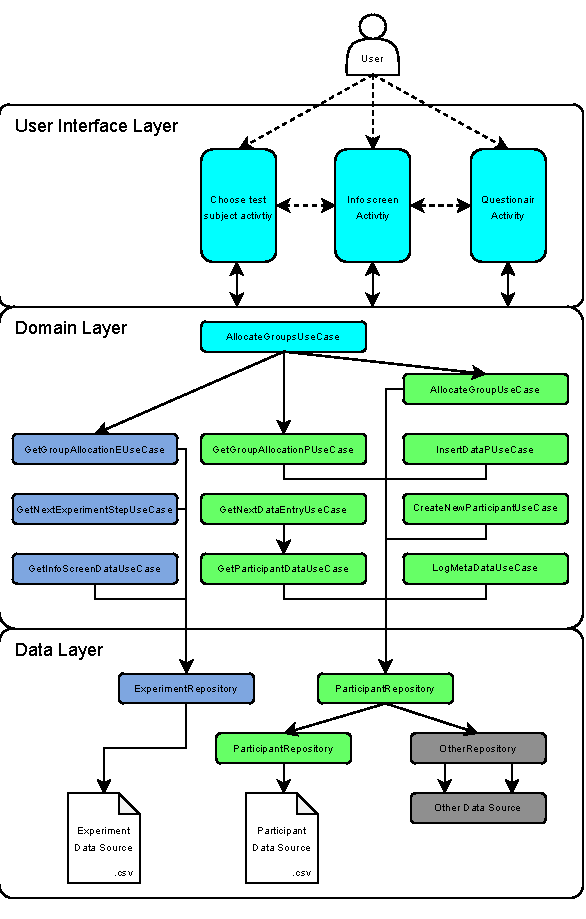
\includegraphics[width=0.79\textwidth, keepaspectratio]{content/05_design_and_dev_artefacts/Complete Architecture.drawio.pdf}
    \caption{Complete Architecture of the Artifact}    
    \label{fig:completeArchitecture}
\end{figure}